\part{Quinto semestre}
\chapterimage{6.pdf} % Chapter heading image
\chapter{Administración Agropecuaria}
\section{Introducción}
La importancia de la administración 

Se aplica en todos los niveles de la sociedad: familias y organizaciones; no existe una historio fidedigna, sistemática; las prácticas administrativas de inician cuando los seres humanos se unen para emprender proyectos no posibles para una sola persona; el paso a la vida sedentaria, permite el surgimiento de la administración pública para prestar servicios de salud, seguridad, drenaje, agua, etc.Los antecedentes de prácticas administrativas son de instituciones religiosas; existieron libros de impuestos, deudas y cuentas por cobrar; La invención de la escritura tuvo más causas económicas y administrativas que religiosas hace 7,000 años.

Para poder construir las diferentes maravillas del mundo antiguo, se requirió de un complejo sistema de administración (a manera de ejemplo la pirámide de Keops abarca $4000m^2$, dos millones de bloques de piedra y 100,000 hombres durante 20 años). Los griegos, un pueblo democrático por excelencia, desarrollaron un nuevo tipo de gobierno ``La polis'' que alentó el libre intercambio de ideas. Los principios de administración reconocieron que la producción máxima es alcanzada mediante el uso de métodos uniformes a tiempos estipulados. Donde el trabajo era repetitivo, la flauta y el clarinete gobernaron los movimientos, con sonidos para cada tarea y para cada operación. ¿Quién hace el aporte de la división del trabajo? Ninguna cantero afilaba su herramienta, Platón llegó a establecer que ningún hombre debería trabajar simultáneamente la madera y el hierro, ya que así no descollaría. Se hace mejor y fácilmente cuando un hombre hace una cosa en armonía con su habilidad y en el momento oportuno.\cite{taylor1973principios}

El significado de la revolución industrial en el desarrollo de la diciplina administrativa
\begin{itemize}
    \item 1760-1830 en países como: Inglaterra, Estados Unidos, Francia, Alemania, etc.
    \item Consistió en la sustitución de la fuerza humana por la máquina en el proceso de producción de bienes 
    \item Es un periodo de sustitución de las relaciones de la producción feudal por las relaciones capitalistas
\end{itemize}

En éste entonces habían \textbf{empresas descentralizadas} que consisten en la concentración del trabajo de un número considerable de obreros que viven en el campo, que realizan el acopio de productores y que en una planta concentradora son sometidos a un proceso de terminado para adquirir el sello de la producción capitalista la homogeneidad, la estandarización y \textbf{Las empresas centralizadas} que consiste en grandes locales en cuales reúnen a una gran cantidad de obreros a quienes someten a una vida de cuartel, este tipo de organización era considerado indigno.

Las innovaciones técnicas son la utilización del coque en la fundición de hierro cuyo proceso mejora la calidad y resistencia; la construcción de los primero altos hornos, la máquina para bombeo de agua que permite elevar el agua y caer y hacer girar una rueda se genera energía eléctrica; las máquinas hiladoras que incrementan aceleradamente la producción y los procesos de blanqueo, estampado y coloración hacen surgir la química moderna.

Las innovaciones financieras y la ética protestante: El tamaño de las corporaciones, un sólo dueño, la imposibilidad de conseguir socios, crédito para crecer, responder a las deudas con los bienes de la empresa, pero con los de la familia también; el papel de los bancos para el crecimiento y para la disminución de las tasas de interés; los seguros en la disminución del riesgo a pérdidas por siniestros.
\begin{itemize}
    \item Piensas que el tiempo es dinero
    \item Piensa que el crédito es dinero
    \item Piensa que el dinero es fértil y productivo
    \item Un buen pagador es dueño de la bolsa de cualquiera
    \item Nada contribuye a hacer progresar en la vida de un hombre joven como la puntualidad y la justicia en todos sus negocios
    \item El golpear el martillo sobre el yunque oído por tu acreedor a las cinco de la mañana o a las ochos de la tarde, lo deja contento por seis meses
    \item El que disipa parte de su tiempo por valor de un céntimo
\end{itemize}

\emph{``Los EUA constituyen el verdadero campo de actividad de la raza humana. Son la esperanza y el asilo de los oprimidos y de los atropellados en otras latitudes. El ejemplo sin par entre las naciones de la tierra, la estrella más brillante del firmameno político, que está aliviando la pesada carga de la aristrocacia y promueve un espíritu democrático en todo el mundo'' M. Weber}

% 30 años pa pensionarse en Chapingo 

La dinámica del capitalismo, es que el patrón ofrece un puesto de trabajo y el obrero está en libertad de aceptarlo o rechazarlo, en la revolución industrial la incorporación de las máquinas, potencia la productividad del trabajo. El proceso de trabajo se secciona en partes ínfimas contra cuándo el trabajador era admirado por la consecución de la terminación de un producto; hoy es sólo apéndice de la máquina. Hace una tarea cuyo producto es para otro pero más aún, el ritmo e iniciativa no le pertenece, sino que es un mejo ejecutor de tareas.
% El control formal y control real
\subsubsection{Prácticas empresariales para aumentar la ganancia}
Para disminuir costos, utilizaban a los niños como bestias de tiro en las minas, por hacer uso de la energía de mujeres y niños, los exentaban hasta por 10 años de pagar impuestos (los libraban de vicios), la reducción de la jornada laboral era exponer a los trabajadores a vicios y actividades fuera de la buena moral; las reacciones de los trabajadores fueron huelgas, afiliarse a sindicatos, destruir la maquinaria para evitar despidos; Todas estas actividades fueron calificadas por los empresarios, el gobierno y la sociedad dominante como atentatorios contra la OD, las buenas costumbres y la ley.

Los protagonistas del modo de producción capitalista:
\begin{itemize}
    \item Los empresarios detentan el capital, los medios de producción y del conocimiento, y echan mano de un nuevo tipo de trabajador para garantizar el éxito del capital adelantado, surge una disciplina la administración y el administrador
    \item Los trabajadores al ser concentrados en un sólo local son organizados por necesidades del capital y ello propicia se organicen para defenderse, para mejorar como clase social
\end{itemize}
Los socialistas utópicos son Robert Owen, Charles Fourier y Saint Simon, rescataron bien las características de sobre explotación:
\begin{itemize}
    \item Deshumanización del sistema y lo parcial del accionar del estado a favor de la clase poseedora del capital y de los medios de producción
    \item Por ello proponían una sociedad igual para todos donde el estado se convirtiera en verdadero árbitro de las relaciones de la sociedad.
\end{itemize}
Carlos Marx, estudia las relaciones del capitalismo de manera objetiva y científica. Explica de manera diferente la existencia de ricos y pobres.

M. Weber que lo explica por la posposición del goce, la frugalidad y la dedicación al trabajo al trabajo

C.Marx lo explica esa situación a la acumulación originaria de capital, mediante una brutal expropiación y posterior explotación de los burgueses a los campesinos pobres; sobre todo a la salvaje, irracional e intenso saqueo de las riquezas coloniales, de metales preciosos y productor útiles a la industria capitalista; pero van más allá la trata de personas implantando un neo-esclavismo. En las relaciones capitalistas maduras C. Marx adjudica al trabajo vivo la virtud de la reproducción ampliada

La posición de la iglesia ante el funcionamiento de las relaciones de producción capitalista:
\begin{itemize}
    \item Se pronuncia ante la sobre-explotación de los trabajadores: para proteger a sus feligreses, porque pagan diezmos, primicias y limosnas, y para frenar al socialismo
    \item Los pronunciamientos de la iglesia se encuentran en las encíclicas, la más importantes fueron: \begin{itemize}
        \item Rerum novarum, el papa León XVIII considera que hay que proteger a los trabajadores ya que sin culpa alguna se han quedado en la miseria mientras que los empresarios son inmensamente ricos
        \item Se pronuncia en contra de la colectividad de la tierra porque dios no dio la tierra en común sino en base  a laboriosidad y cada sociedad determinará que le toca a cada quién y el estado no debe intervenir sino vigilar la convivencia de las personas.
    \end{itemize}
\end{itemize}
\subsubsection{Sistematización de la administración}
\begin{itemize}
    \item Teoría clásica (AC) inician la sistematización de la administración: Frederick Winslow Taylor y Henry Fayol (1911-1912 y 1916)
    \item La utilidad de la administración como diciplina útil y necesaria (Para garantizar el éxito del capital adelantado)
    \item Con la disciplina sistemática surge el administrador profesional, para mediar la relación KL para sustituir con ventaja al dueño del capital
    \item F.W. Taylor inicia con un diagnóstico de la situación presente; estado de cosas de la producción, el comportamiento obreros y el de los sindicatos 
\end{itemize}

La administración Científica no es ningún plan de eficiencia, ni una especie de programa para asegurar la competencia, ni es un grupo de proyectos eficientes, no es un estudio de tiempos, no es un estudio de movimientos, no es dirección dividida, 
\begin{definition}[Administración Científica]
    Es una revolución mental completa por parte de los trabajadores de cualquier establecimiento o industria, una revolución mental completa, por parte de estos hombres en cuanto a sus deberes respecto a su trabajo, a sus compañeros y a sus patrones. E implica una revolución mental igualmente completa por parte del sector directivo y del propietario en cuanto a sus obligaciones hacia sus compañeros de trabajo en la administración, hacia sus obreros y hacia todos los problemas diarios de estos.
\end{definition}
Para aclarar el concepto anterior, se describe la situación empírica:
\begin{itemize}
    \item Tanto empresarios como trabajadores se centran en luchar por apropiarse del mayor porcentaje del superávit
    \item Estos conflictos han conducido a grandes desencuentros y huelgas donde se ven como enemigos y enfrentan sus fuerzas
    \item Da fin a la lucha de clases planteada por Marx: \emph{Vuelven su atención hacia el aumento de las dimensiones del superávit hasta que es tan grande que es innecesario pelear por su división}
    \item Son capaces de hacer este superávit tan enormemente mayor de lo que era en el pasado, que existe amplio margen para un gran aumento de salarios para los trabajadores y un crecimiento similar de beneficios para el fabricante
\end{itemize}
En un inicio dice que no es AC, y busca un camio de actitud en los protagonistas de la producción capitalista; pero en cuanto esta revolución mental se ha dado, no hay aún AC, hay que implementar todo los que al inicio señala (no es la AC)

Entonces en concreto, para Taylor para que existe administración Científica deben cumplirse dos condiciones:
\begin{itemize}
    \item Obligación para cooperar al engrandecimiento del mayor superávit posible 
    \item y la necesidad de substituir las opiniones o la vieja regla del conocimiento burdo e individual
\end{itemize}

\subsubsection{Principios de administración H. Fayol}
Reconoce que la administración sólo tiene que ver con el personal y no con el resto de la empresa: producción y seguridad\dots
También señala que no debe haber rigidez sino justa proporción dependiendo de la experiencia y criterio del administrador
\begin{enumerate}
    \item División del trabajo: entre más madura una organización más diferenciada, el objetivo de este principio es producir más y mejor
    \item Autoridad y responsabilidad: el derecho de dar órdenes y esperar obediencia: diferenciar entre autoridad formal
\end{enumerate}

\subsubsection{Variables económicas}
Los Paquetes tecnológico, diseño, procesos y la ley que regula el sector: son los factores que determinan los procesos de producción, de esta manera tendremos los dos contextos.
\begin{enumerate}
    \item \textbf{Contextos estables}: Dependen que en mucho tiempo han estado conviviendo con el paquete tecnológico (una sola variables)
    \item \textbf{Contextos cambiantes}:El cambio puede ir por cualquiera de las cuatro variables
    \item \textbf{Contextos turbulentos}: No se sabe qué variable hará el cambio,
\end{enumerate}
Un administrador es quien realiza es

Los gerentes tienen un posición en el organigrama y no necesariamente tiene una actitud de liderazgo pero es una persona que puede premiar o castigar, respaldo legal; los líderes no necesariamente tienen poder pero ejercen liderazgo es decir que es respetado por su experiencia, consejos, carisma, poder de referencia, 

Para administrar el contexto, hay que hacer proactivo (Aquel que ha visto problemas antes de ocurrir), los reactivos son visionarios que ven a corto plazo con problemáticas actuales.
\begin{definition}[Industria]
    Conjunto de productores de bienes o servicios
\end{definition}
La conversión de la materia prima a materia terminada no es una definición precisa para la industria
sectores industriales: sector embrionario se pone barreda de entrada (Una patente) ellos escriben las reglas a tu favor
sectores fragmentados: consolidar el sector es que un grupo de productores se dividen en diferentes actividades (Se reduce el número de oferentes)
Sector global: es un único precio, 

% misión: qué hacer cómo y para quién
% visión: la imagen futura de la empresa, se le agrega el año
% \footnote{Tipo de Empresas: domésitcas regionales nacionales internacionales trasnacionales y mundiales.}

\subsection{Globalización}
\begin{definition}[Globalización]
    Concentración de capitales en pocas manos, es un proceso agresivo de un poder global, el sistema mundo se hace poderoso con respecto a las naciones.
\end{definition}
Los criterios de calidad en agricultura son:
\begin{itemize}
    \item Color, color de la cascara
    \item Peso
\end{itemize}
Éstos productos con la mejor calidad tienden a exportarse a los países más poderosos.
\subsection{Contexto organizacional}

Las características de las escuelas: clásica, neoclásica, estructuralista con respecto al contexto. Todas estas escuelas que son dominantes, no daban importancia al ambiente externo de la organización, se centraban en el ambiente interno y en la búsqueda de eficiencia y no en la eficacia.

El contexto externo de la organización puede ser definido como el conjunto de variables que están fuera de la organización pero que afectan el desempeño de la misma, creando un clima, ante el cual la organización se adapta, responde o se anticipa.
\begin{center}
    \smartdiagram[connected constellation diagram]{Organización y sus gerentes,Junta de accionistas,Oferta de mano de obra,Instituciones gubernamentales,Instituciones financieras, Proovedores,Competidores, clientes}
\end{center}
\begin{center}
    \smartdiagram[bubble diagram]{
    Organización,Variables \\ tecnológicas,Variables \\socio culturales,Variables \\político legales,Variables \\económicas}
\end{center}

\subsubsection{Variables tecnológicas}
\begin{itemize}
    \item Sucesos en otras industrias
    \item Investigación y desarrollo
    \item En caso de México: tintes naturales, el algodón y el henequén
    \item El cobre vs fibra óptica
\end{itemize}
\subsubsection{Variables político-legales}
\begin{itemize}
    \item Grupos políticos de presión
    \item Clase empresarial
    \item Los partidos políticos
    \item Comportamiento en otros países
    \item Legislación
\end{itemize}
\subsubsection{Variables socio-culturales}
\begin{itemize}
    \item Grupos educativos
    \item Grupos ecológicos
    \item Medios de comunicación
    \item Formas de organización
    \item Formas de convivencia
    \item Formas de consumo
\end{itemize}
\subsubsection{Variables económicas}
\begin{itemize}
    \item Comportamiento del PIB
    \item La inflación 
    \item Tipo de cambio
    \item Precio del petróleo
    \item Turismo
    \item Política fiscal
\end{itemize}
\subsubsection{Organización y sus responsabilidades con la sociedad}
Milton Friedman: Las organizaciones sólo deben dedicarse a la producción eficiente de productos y servicios. Otros teóricos: los negocios deben cuidar una imagen ante la sociedad y, no interesarse por los problemas sociales es suicidarse en largo plazo.
\subsubsection{Relaciones entre estructura- estrategia y medio ambiente}
Las empresas reactivas y su ambiente, donde el proceso de formulación de estrategia tiene que considerar al ambiente en que opera en la actualidad y en el que operará en el futuro. Las empresas proactivas: donde el proceso de formulación de estrategia implica elegir el ambiente en que la empresa va a operar en el futuro

Dentro del ambiente internacional, está el contexto externo de las cuatro variables vistas; de aquí derivan las amenazas, oportunidades y estrategias. Pero en el ambiente interno derivan las fortalezas y debilidades, objetivos, valores, creencias, y la estrategia
\emph{Los cambios en la estrategia de la sociedad anónima preceden y conducen a cambios en el diseño organizacional\cite{chandler1962strategy}}
\subsubsection{Influencia de la estrategia en la estructura de la organización}
Determina las tareas organizacionales, que son la base del diseño de la empresa. Influye en la elección de tecnología y de las personas afectadas para desempeñar las tareas y determina la estructura. Determina el ambiente específico dentro del cual va a operar la organización, esto también influye en la estructura
\subsubsection{Clasificación de ambientes organizacionales}
\textbf{Estable:} Un ambiente estable es cuando está libre de cambios inesperados o súbitos, los cambios se pueden planear con bastante anticipación, la demanda de mercado sólo muestra pequeñas fluctuaciones previsibles. Las leyes que afectan a la industria han estado en vigor durante largo tiempo y no hay señales de que vayan a cambiar. No se esperan innovaciones tecnológicas, por los presupuestos en investigación son mínimos o no existen. Hoy por lo general, no existen los ambientes estables.

\textbf{Cambiantes:} La innovación puede aparecer en cualquiera de las áreas (producto, mercado, legislación o tecnología). pero estos cambios no causan sorpresas en la alta dirección ya que las tendencias son visibles y se pueden predecir y, las empresas se adaptan con facilidad.

\textbf{Turbulento:} Cuando los competidores lanzan inesperadamente nuevos productos, cuando se aprueban leyes sin previo aviso y cuando un invento tecnológico revoluciona de pronto el diseño o el método de producción, la organización se encuentra inmersa en un ambiente turbulento.

\subsubsection{Objetivos organizacionales}
\begin{center}
    \begin{tikzpicture}
        \coordinate (A) at (-5,0) {};
        \coordinate (B) at ( 5,0) {};
        \coordinate (C) at (0,7) {};
        \draw[name path=AC] (A) -- (C);
        \draw[name path=BC] (B) -- (C);
        \foreach \y/\A in {0/Objetivos individuales,1/Objetivos de departamento,2/Objetivos de división,3/Objetivos de áreas clave,4/Objetivos estratégicos,5/Misión,6/Propósito Socioeconómico} {
            \path[name path=horiz] (A|-0,\y) -- (B|-0,\y);
            \draw[name intersections={of=AC and horiz,by=P},
                  name intersections={of=BC and horiz,by=Q}] (P) -- (Q)
                node[midway,above] {\A};
        }
    \end{tikzpicture}
\end{center}
Los tres pisos más altos en la cúspide, están a cargo el Consejo de administración, del tercero al sexto está el Director General, del segundo al cuarto los Mandos Medios y los primeros dos escalones son Gerentes Operativos. Por un lado está la comunicación ascendente (De menor a mayor puesto) y homólogamente la comunicación descendente.

Los objetivos organizacionales son:
\begin{itemize}
    \item El concepto
    \item Tipos: Estilísticos-rendimiento
    \item Ideal inalcanzable
    \item Objetivo del empresario vs el objetivo de los trabajadores
    \item Falsos consensos
\end{itemize}
Procesos de formación de objetivos:
\begin{itemize}
    \item Procesos de formación de alianzas y regateo o fijación de objetivos de la coalición
    \item Fase de control mutuo, de acuerdo a la correlación d fuerzas
    \item Procesos de adaptación a la nueva situación
\end{itemize}
Otros pagos para hacer viables los objetivos organizacionales, son con pagos colaterales

CEO (Chief Executive Officer): Es una persona que tenga la responsabilidad en la conducción de personas y manejo de recursos organizacionales, existen diferentes habilidades en un líder:
\begin{center}
    \smartdiagram[descriptive diagram]{
    {Técnica,Capacidad de usar herramientas, procedimientos o técnicas en un campo especializado},
    {Humanas, {Es la habilidad de trabajar con otras personas, de comprenderlas y motivarlas}},
    {Conceptuales, Es la habilidad mental de coordinar e integrar todos los intereses y actividades de la organización},
    {Diseño, {La capacidad para detectar oportunidades de negocios, para la organización}},}
\end{center}
Es un verdadero mito que las IES puedan preparar al 100\% al gerente. Les enseñan a resolver problemas, deberían enseñarles a detectar nuevas oportunidades de negocio, es un mito el gerente bien preparado:
\begin{itemize}
    \item La necesidad de administrar: asumir y buscar responsabilidad en la administración de recursos organizacionales
    \item Necesidad de poder: Capacidad para influir en el comportamiento de otros
    \item Capacidad de empatía: Comprender y canalizar las aspiraciones no expresadas de las personas para conseguir los objetivos organizacionales, de grupo e individuales
\end{itemize}
\begin{table}[h!]
    \centering
    \begin{tabular}{@{}cc@{}}
    \toprule
    Mitos &
      Realidades \\ \midrule
    \begin{tabular}[c]{@{}c@{}}El directivo es un\\ planificador reflexivo y\\ sistemático\end{tabular} &
      \begin{tabular}[c]{@{}c@{}}Hacen trabajos, breves y discontinuos que\\ están muy orientados a la acción y no les\\ gustan las actividades reflexivas\end{tabular} \\
    \begin{tabular}[c]{@{}c@{}}El directivo eficaz no tiene\\ que realizar obligaciones con\\ regularidad\end{tabular} &
      \begin{tabular}[c]{@{}c@{}}Además de tratar las excepciones el trabajo\\ del directivo implica la ejecución de varias\\ obligaciones regulares, incluyendo los rituales y\\ ceremonias, procesar información blanda que\\ enlaza a la organización con su entorno\end{tabular} \\
    \begin{tabular}[c]{@{}c@{}}El alto directivo necesita\\ que la información esté\\ resumida,, lo que consigue\\ mejor mediante un sistema\\ formal para la dirección\end{tabular} &
      \begin{tabular}[c]{@{}c@{}}Los directivos prefieren los medios orales\\ (llamadas telefónicas, reuniones programadas y\\ no programadas, paseos de observación)\end{tabular} \\
    \begin{tabular}[c]{@{}c@{}}La dirección es o por lo\\ menos se está convirtiendo,\\ rápidamente en una ciencia y\\ una profesión\end{tabular} &
      \begin{tabular}[c]{@{}c@{}}Los programas de los directivos, programar\\ el tiempo, procesar información, tomar\\ decisiones, y así sucesivamente permanecen\\ encerrados en sus cerebros, en base a\\ conceptos como juicios e intuición\end{tabular} \\ \bottomrule
    \end{tabular}
    \caption{Mitos y realidades sobre los directivos}
    \label{tabaa1}
\end{table}
\begin{table}[h!]
    \centering
    \begin{tabular}{@{}ccc@{}}
    \toprule
    Interpersonales &
      Informativos &
      Decisorios \\ \midrule
    \begin{tabular}[c]{@{}c@{}}Cabeza visible\\ Líder\\ Enlace\end{tabular} &
      \begin{tabular}[c]{@{}c@{}}Monitor\\ Diseminador\\ Portavoz\end{tabular} &
      \begin{tabular}[c]{@{}c@{}}Empresario\\ Solucionador de conflictos\\ Asignador de recursos\\ Negociador\end{tabular} \\ \bottomrule
    \end{tabular}
    \caption{Papeles del gerente que le dan autoridad formal y status}
    \label{tabaa2}
\end{table}
Tipos de conocimientos: 
\begin{itemize}
    \item Conocimiento empaquetado: libros, videocassette
    \item Conocimiento migrante: intercambios culturales, estancias en el extranjero, estancias de extranjeros, estudios de posgrado
    \item Conocimiento insertado: Experiencia, capacitación, formación de grupos interdisciplinarios y autoríwgidos
\end{itemize}
% La competitividad de una institución se determina por:
% \begin{itemize}
%     \item Eficiencias de las empresas: Rendimiento de la creación de empresas
%     \item Eficiencia de gobierno: Rendimiento con la colaboración del gobierno
%     \item Dotación de infraestructura: Cuánta infraestructura hay
%     \item Índice de formación de cerebros: Cuántos tienen maestría
% \end{itemize}
% La organización de una organización gerencial:

% El trabajo gerencial planea estrategias pero coordina procesos cortos; el gerente se basa en sus informante clave; 
% \begin{itemize}
%     \item Primera línea
%     \item ápices
%     \item a?
% \end{itemize}
% Se dice que la administración es una mezcla de ciencia técnica y arte; realizar las cosas a través de otros,    
% \begin{definition}[Adminsitración]
%     La ley de la partida doble: ``A todo cargo corresponde un bono''.
% \end{definition}

% Trabajo simple es la capacidad de trabajar sin preparación; el trabajo complejo,
Características de la sociedad del conocimiento: Quioscos activados por voz para recoger el periódico sin tocar nada, robots a las entradas de los hoteles para recibir a los turistas y hologramas que sustituyen a los botones para reducir el contacto en los ascensores. Son algunos ejemplos del tipo de soluciones tecnológicas en las que ya se está trabajando para hacer frente al mundo que se presenta tras la crisis del coronavirus.

La definición de sociedad del conocimiento para México implica que tanto individual como colectivamente los individuos tienen capacidad para:
\begin{itemize}
    \item Apropiarse del conocimiento que se genere en cualquier parte del mundo
    \item Aprovechar de la mejor manera el conocimiento que esa sociedad ha producido históricamente, incluyendo conocimiento científico y tecnológico, y también los conocimientos locales y tradicionales
    \item Generar por ellos mismos los conocimientos que les hagan falta para comprender mejor sus problemas (educativos, económicos, de salud, sociales ambientales, etc.) para proponer soluciones y realizar acciones, para resolver efectivamente; por tanto una sociedad del conocimiento debe ser justa, democrática y plural
\end{itemize}
\begin{definition}[Conocimiento]
    Un conjunto de exposiciones ordenadas de hechos e ideas, que presentan un juicio razonado o un resumen experimental, que se trasmite a otros a traves de algún medio de comunicación bajo una forma sistemática
\end{definition}
Aspectos característicos:
\begin{itemize}
    \item Apropiación privada del conocimiento y sus frutos, por medio de patentes y copyright
    \item La nueva élite se distinguirá de la masa, por el tipo de institutos que las expidan
    \item La política futura se basará en los intereses de la sociedad comunal
\end{itemize}

\subsubsection{Sociedad del conocimiento}
Según Peter Drucker (1959) en su libro \textit{revolución educativa}, el trabajo manual se volverá improductivo en comparación con el trabajo conceptual.

La educación se constituye en medio de reflexión y propuesta. Sin embargo existen ciertas preocupaciones:
\begin{enumerate}
    \item Desigualdad derivada del éxito diferencial de los sujetos altamente educados: Desplazar la atención de recompensas económicas y buscar la manera de volverlos significativos y satisfactorios
    \item Crecientes desigualdades de riqueza derivadas de la desigualdad educativa internacional: Que la cooperación internacional brinde apoyo. Sugerencia de Costa Rica
\end{enumerate}

El crecimiento del papel de la ciencia, la tecnología y el conocimiento, como modelo deseable
\begin{center}
    \smartdiagram[Sociedad Postindustria]{
        Sector económico,En la distribución ocupacional,COmo principio axial,Como oriental futura,Para la toma de decisiones
    }
\end{center}
Se dan una nueva clase de elitistas, egoístas, de idiologías de profesionalismo o está el grupo de inteligencia técnica contra los que controlan la economía; se da una nueva lucha de clases para controlar la situación laboral.

Existen ventajas como principio organizativos:
\begin{itemize}
    \item Su aplicación no supone desgaste, si no multiplicación
    \item Su producción requiere creatividad, la libertad de circulación y los intercambios
    \item Desde el punto de vista organizativo
\end{itemize}

\subsubsection{Estructura ocupacional}
Hay tres grupos:
\begin{itemize}
    \item Rutinarios \begin{itemize}
        \item Fábricas
    \end{itemize}
    \item Personales \begin{itemize}
        \item Empleados de hoteles
        \item Vertedores
    \end{itemize}
    \item Simbólicos \begin{itemize}
        \item Diseñadores
        \item Ingenieros
        \item Científicos
    \end{itemize}
\end{itemize}
¿Qué pertinencia para America latina? los factores que impiden el crecimiento equilibrado del sistema científico técnico son las migraciones, no tienen condiciones laborales para los cientificos, migraciones temáticas, decada de los 80 y 90 división de actividades por países y regiones; y desigualdad de oportunidad entre hombres y mujeres.

La sociedad del conocimento, es una sociedad imaginada y regida por la lógica de producción y acumulación de conocmientos, para sustituir a sociedades con problemas y realidades concretas muy diversas. Esta es la opción adecuada para eld esarrollo de América Latina y de otros países pobres, para logarle falta mucho en que trabajar.

% \subsection{Técnica PERT}
% Program Evaluation and Review Technique (PERT) y Critical Path Method (CPM), al final de la segunda guerra mundial se usaron como herramienta de planificación con la gráfica de Gantt, actividad vs tiempo

\section{Globalización}
\begin{definition}[Globalización]
    Una definición única de la globalización, válida para todo el mundo no existe porque se tienen muchas ideas distintas sobre lo que es.

    Es la perceptible pérdida de fronteras del quehacer cotidiano en las distinas dimensiones de la economía, la información, la ecología, la técnica, los conflictos transculturales y la sociedad civil. (Beck, 1998 en Rodríguez Miguel J.C., 2009\cite{bini2009coefficient})

    La interdependencia económica creicente en el conjunto de los países del mundo, provodada por el aumento del volumen y de la variedad de las transacciones transfronterizas de bienes y servicios, así como de los flujos internacionales de capitales, al mismo tiempo que por la difusión acelerada y generalizada de la tecnología (FMI en Ramiro Mateus J et al. s,f\cite{mateus2002globalizacion})

    La interdependencia económica creciente en el conjunto de los países del mundo, provocada por el aumento del volumen y de la varidedad de las transacciones transfronterizas de bienes y servicios, así como de los flujos internacionales de capitales al tiempo que la difusión acelerada y generalizada de tecnología
\end{definition}
En conclusión: ``Internacionalización del capital financiero, industrial y comercial, donde las telecomunicaciones y la informática, especialmente el internet, jugaron un papel decisivo en la construcción de un mundo cada vez más interconecado, en una aldea global''

Interrelación e interconexión; trabajar como una unidad, en tiempo, a escala planetaria, a travpes de redes de interconexiones.

Palabras vinculadas al concepto de globalización

Palabras vinculadas al concepto de globalización:
\begin{definition}[\% Extensión]
    simple extensión física o tecnológica" una extensión global de las relaciones sociales entre los seres humanos (más espacio).
\end{definition}
\begin{definition}[Intensificación]
    Intensificación de las relaciones globales de interacción e intercambio" [...] entre estados, sociedades y resto de agentes que operan a escala mundial". Schriewer (1996) (más fuerte, enérgico o activo algo).
\end{definition}
\begin{definition}[\% Interdependencia]
    No existen personas aisladas, ni grupos incomunicados; no hay ningún país que pueda vivir al margen de los demás; no existen espacios cerrados, porque está todo interconectado, y todo lo que sucede afecta a todos y a cada uno de los seres humanos- Los transportes y las nuevas tecnologías de la información y la comunicación, han hecho que el mundo se haga más pequeño.
\end{definition}
No existe una geniuina globalización como referencia a un único proceso lineal y homogéneo.
\subsubsection{Dimensiones fundamentales de la globalización}
\begin{enumerate}
    \item \textbf{Dimensión económica:} Conjunto de procesos de tipo económico que se desarrollan nivel mundial, dando respuesta a las demandas del mercado, ovedeciendo al mismo tiempo las reglas que lo forman y las organizaciones que las manejan. Propicia el libre comercio y la libre circulación de capital. Un mercado capitalista y sus empresas multinacionales.
    \item \textbf{Dimsensión política:} Reducción de poder de los Estados-nación, perdiendo parte de su soberanía en favor del mercado. Resiente la capacidad de los estados de representar a sus ciudadanos y defender sus derechos y el sentido y significado del proceso democrático. Provoca, por último, que la política y las decisiones sean cada vez más internacionales y que dichas políticas estén en gran parte controladas por organismos internacionales de carácter económico y grandes empresas privadas. Relacionándola con la finalización de la ``guerra fría'' y el nuevo papel que desempeña la Organización de las Naciones Unidas ``gobierno mundial''.
    \item \textbf{Dimensión cultural:} Las sociedades hacia un uniformismo cultural y hacia el pensamiento único, apoyándose en los medios de comunicación y de difusión cultural, y en el comercio de productos. y servicios. Universalización de determinados modelos de valor; por ejemplo, el reconocimiento general de los principios liberal democráticos y de los derechos fundamentales; la generalización del modelo de consumo capitalista. Este desarrollo se vincula fuertemente con la formación de monopolios de los medios de comunicación de masas.
    \item \textbf{Dimensión ecológica:} Hace referencia a los peligros que para las sociedades representan los daños ecológicos. Los cuales ya no tienen una repercusión local, sino global (Stiglitz en Rodríguez. Miguel J.C, 2009). También esta dimensión provoca el avance positivo de los procesos de concienciación mundial sobre cuidado del planeta y hace más visible el proceso de globalización y las interdependencias y efectos causales a nivel mundial, que tienen las agresiones contra el medio ambiente.
    \item \textbf{Dimensión social:} La globalización ataca a la sociedad debilitando el grupo en favor del individuo, provoca la exclusión y la fragmentación social, intenta debilitar o hacer desaparecer derechos fundamentales (laborales, de educación, de salud, etc.) a favor de su privatización, provoca que las sociedades estén más interconectadas y sean más interdependientes, y que las mismas se constituyan en sociedades de la ``información'' o el ``conocimiento''
    \item \textbf{Dimensión Psicológica:} Produce una influencia negativa sobre la estabilidad psicológica y la personailidad de los sujetos, así como el aumento y extensión de ciertos trastornos, además de la aparición de otrs nuevas formas de hacer negocios.
\end{enumerate}
Hay una conseiencia medioambiental sobre el planeta y sus recursos; y por la inconsciencia y la falta de medidas ecológicas de estados y corporaciones transnacionales ante los mismos.

Así mismo hay una destrucción de la soberanía alimentaria: la globalización, los grandes monopolios que la impulsan hace que se creen zonas de monocultivos que destruyen la diversidad, necesaria, de países sobre todo pobres. Además el control de la alimentación cada vez está en menos, grandes empresas controlan el comercio y los productos, creando transgénicos.
\subsection{Evolución de la disciplina administrativa}
Escuela Científica F.W. Taylor ¿Qué es la administración científica?, Estracto del testimonio de la FWT en la Audiencia en la Comisión Especial de la cámara de representatnes para investifar el sistema de Taylor y otros de administración de talleres.

\subsubsection{Escuela Científica}
La ac es una revolución mental completa por parte de los trabajadores de toda org, o industria, una revolución mental de esos hombres respecto a sus deberes. su trabajo, sus compañeros y sus patrones. Tambniéne s una revolución mental completa de los administradores, los directivos y los dueños acerca de sus deberes, su trabajo, sus trabajadores.

En el pasado: los empresarios buscaban mayor rentabilidad, los obreros buscaban mayores salarios; esto es, la división del superavit.

El costo de venta se le resta, el costo de las materias primas, salarios, maquinaria luz renta del edificio; todo esto son los costos de producción, si se restan al precio de venta, lo que queda es el superavit. 
\begin{definition}[Superavit]
    Ganancia del empresario y salarios de los trabajadores, en esto se centraba la relación $k-l$
\end{definition}
Cuando disminuyen la venta, el empresario baja los salario spara conservar sus ganancias, el trabajador quieren el salario y sus aumentos cotidianos: expresión de la lucha de clases sociales es definición de una epoca de crisis

¿Cómo opera la gran revolución mental de la AC?
\begin{itemize}
    \item Ambas clases despegan su visión de la división del superavit como cuestion primordial y ambas se centran el auento del mismo, hasta que este es tan grande que es innecesario pelear por la división de el
    \item Descubren que si dejan de pelear por su división, y secentran ambos en su aumento los resultados son expectaculares
    \item Esto significa la sustitución de la guerra por la paz, en ves de ser recelosos se dan confianza mutua, en concreto, dejan de ser enemigos y son amigos, a partir de aquí se puede desarrollar la AC
    \item hasta el cambio de la gran rev mental completa, es positivo pero aun no pasa nada, no existe nada concreto, falta implementar los buenos anexos, pero que no es la AC
\end{itemize}

\subsubsection{Administración como profesión}
Administración científica
\begin{itemize}
    \item Preocupada de la técnica administrativa y de la técnica de funcionamiento
    \item Administración especializada o funcionalizada, diferentes tipos de problemas, conjuntos de conocimiento
    \item Disminución de la autoridad arbitraria (valor al método científico), investir de autoridad a la persona con más conocimiento y más habilidad para aplicar ese conocimiento.
\end{itemize}
Experiencias del liderazgo: Predidente y expertos diversos.

Para la administración de empresas, el adiestramineto está ganando importancia sobre la simple personalidad, hace falta más ciencia para comprender a los seres humanos y sus derechos para plocamar la equidad.

Para el Dr John R. Commons, divide tres épocas históricas:
\begin{itemize}
    \item Era de la escasez
    \item Abundancia
    \item Estabilización: Control consiente y deliberado de las fuerzas económicas en bien del interés social general
\end{itemize}
Cinco pasos para la administración científica:
\begin{enumerate}
    \item Una administración eficaz que ha de ocupar el lugar de aqueñña explotación de nuestros recursos naturales, cuyos días están ahora a punto de acabarse
    \item Competencia más aguda
    \item Escasez de mano de obra
    \item Un concepto más amplio de la ética de las relaciones humanas
    \item La idea creciente de la empresa como un servicio publico que lleva consigp un sentido de respondabilidad para su conducta efectiva
\end{enumerate}
La administración incluye el lado técnico, un conocimiento de producción y distribución; en el lado personal, un conocimiento de como tratar correcta y fructuosamente con los propuos compañeros.

Una de las primeras cosas para hacer más científica es aplicar métodos científicos, además de hacer un análisis de labores del administrador, que correspondan al análisis de las labores de los trabajadores de Taylor.

Lueo se debe adoptar la administración de empresas es organizar.

Un inconveniente grave para un entendimiento y una utilización mas completos de la experiencia directiva, es que en el presente no tenemos:
\begin{itemize}
    \item Continuidad sistemática de decisiones, de métodos nuevos, de experimentos administrativos,
    \item Ningún sistema de registro elaborado minuciosamente
\end{itemize}
Los registros llevados defectuosamente, la ausencia de ellos, son parcialmente responsables de lo que, en algunas plantas aparece como administración estancada, y en todas ellas, como determinadas fallas administrativas.

Si un directivo esta haciendo frente a determinado problema, debe estar en condiciones de encontrar:
\begin{enumerate}
    \item Si otros directivos han tenido que enfrentarse a problemas similares
    \item Cómo les hicieron frente
    \item Cuales fueron los resultados
\end{enumerate}
Concepto de Planeación Estrategia m: Porter
\begin{enumerate}
    \item Visión
    \item Posicionamiento
    \item Plan
    \item Patrón integrado de comportamiento
\end{enumerate}

\subsection{Matrices de análisis de negocios}
\subsubsection{Análisis de la situación presente }
\begin{table}[h!]
    \centering
    \begin{tabular}{@{}|c|c|c|@{}}
    \toprule
    \begin{tabular}[c]{@{}c@{}}Factores internas\\ Factores externos\end{tabular} &
      \begin{tabular}[c]{@{}c@{}}Lista de\\ fortalezas\end{tabular} &
      \begin{tabular}[c]{@{}c@{}}Lista de\\ Debilidades\end{tabular} \\ \midrule
    \begin{tabular}[c]{@{}c@{}}Lista de\\ oportunidades\end{tabular} &
      \begin{tabular}[c]{@{}c@{}}FO (Maxi-Maxi)\\ Estrategia para maximizar\\ las F y las O\end{tabular} &
      \begin{tabular}[c]{@{}c@{}}DO (Mini-Maxi)\\ Estrategia para minimizar\\ las D y maximizar las O\end{tabular} \\ \midrule
    \begin{tabular}[c]{@{}c@{}}Lista de\\ Amenazas\end{tabular} &
      \begin{tabular}[c]{@{}c@{}}Fa (Maxi-Mini)\\ Estrategia para maximizar\\ las F y minimizar las A\end{tabular} &
      \begin{tabular}[c]{@{}c@{}}Da (Mini-Mini)\\ Estrategia para minimizar\\ las D y las A\end{tabular} \\ \bottomrule
    \end{tabular}
    \caption{La matriz FODA}
    \label{tabap1}
\end{table}
\begin{table}[h!]
    \centering
    \begin{tabular}{@{}ccc@{}}
    \toprule
     &
      \begin{tabular}[c]{@{}c@{}}Igual estrategia\\ que el líder\end{tabular} &
      \begin{tabular}[c]{@{}c@{}}Diferente\\ estrategia que el\\ líder\end{tabular} \\ \midrule
    \begin{tabular}[c]{@{}c@{}}Más recursos que\\ el líder\end{tabular} &
      Ataque frontal &
      Guerra relámpago \\
    \begin{tabular}[c]{@{}c@{}}Meno recursos\\ que el líder\end{tabular} &
      Miniduplica &
      Ataque lateral \\ \bottomrule
    \end{tabular}
    \caption{Matriz 2x2 de Goerge TIP}
    \label{tabap2}
\end{table}
\begin{center}
    \smartdiagramset{planet color=orange!60,
    distance planet-satellite=1cm}
    \smartdiagram[connected constellation diagram]
    {Contextuales o exogenas,Cultura, Tecnología, Economía, Político legal}
\end{center}

\begin{center}
    \smartdiagramset{planet color=orange!60,
    distance planet-satellite=1cm}
    \smartdiagram[connected constellation diagram]
    {Variables\\estructurales,Formalización, Profesionalización\\y especialización, Proporción de\\personal, Estandarización, Complejidad, Jerarquía y\\cnetralización}
\end{center}
\begin{itemize}
    \item Saquean los recursos naturales de comunidades que no conocen el valor de los mismos
    \item Se inmiscuyen en la política de los países receptores
    \item Ensucian el ambiente en países con legislaciones laxas
    \item El discurso de responsabilidad social corporativa no pasa de mera retórica
\end{itemize}
Los elementos mínimos de una organización
\begin{itemize}
    \item Objetivos declarados y dotarse de medios para conseguirlos
    \item Número precisable de miembros
    \item Trato impersonal
    \item Papeles diferenciados
    \item Mecanismos de sustitución de elementos valiosos
\end{itemize}
\subsection{Proceso de toma de decisiones}
Existen muchos modelos de toma de decisiones, según Tersine Richard J. (1973:139), existen seis elementos comunes a toda decisión.
\begin{enumerate}
    \item Agente decisor. Es la persona que hace la escogencia de la opción entre varias alternativas o cursos de acción
    \item \textbf{Objetivos}. Al punto donde el agente decisor pretende llegar con sus acciones
    \item \textbf{Preferencias}. Son los criterios que el agente decisor utiliza para hacer su escogencia
    \item \textbf{Estrategia} Es el curso de acción que el tomador de decisiones escoge para alcanzar mejor sus objetivos
    \item \textbf{Situación}. Son aspectos del ambiente que envuelven al agente decisor, muchos de los cuales están fuera de su control, conocimiento o comprensión y afectan su escogencia
    \item \textbf{Resultado} Es la consecuencia de la estrategia adoptada.
\end{enumerate}
\subsection{Divisiones programadas y no programadas}
\subsubsection{Decisiones programadas}
Son aquellas tomadas de acuerdo a una política, procedimiento o regla, es una toma de decisiones por precedentes. Este tipo de decisiones se aplican a las decisiones programadas limitan nuestras decisiones ya que es la organización y no el individuo la que decide que hacer, es decir existen procedimientos sistemáticos para resolver problemas comunes. Son decisiones programadas cuando existen: Datos adecuados, datos repetitivos, condiciones estáticas, certeza y previsión
\subsubsection{Decisiones no programadas}
Se aplican a situaciones no estructuradas, nuevas y mal definidas de una naturaleza no repetitiva; es decir, si un problema no se ha presentado con suficiente frecuencia para ser incluida en una política o es tan importante que merece un tratamiento especial.

En resumen, la mayor parte de las decisiones no son ni completamente programadas ni completamente no programadas sino una combinación de ambas. Las decisiones no programadas son tomadas por los gerentes de los niveles estratégicos de la organización, porque son quienes tienen que resolver problemas no estructurados; por el contrario, en los noveles inferiores de la organización la toma de decisiones son rutinarias y bien estructuradas y requieren menos libertad por parte de los administradores.
\subsection{Planeación táctica}

Es el conjunto de la toma deliberada y sistemática de decisiones que incluyen propósitos más limitados, plazos más cortos, áreas menos amplias y niveles inferiores de la jerarquía de la organización.

La planeación táctica está contenida en la planeación estratégica y no representa un concepto absoluto, sino relativo: La planeación estratégica general de la organización: es estratégica en relación con cada una de las secciones que componen aquel departamento. 

\subsubsection{Características de planeación táctica}
La planeación táctica tiene diversas características que la diferencia de los tipos de planeación estratégica
\begin{itemize}
    \item Coordina las funciones importantes del organismo
    \item Su realización se enfoca a mediano plazo
    \item Identifica los medios necesarios para lograr los objetivos
    \item Los encargados responsables de la formulación de estos planes, son generalmente principales
    \item Un conjunto de planes tácticos soporta y complementan un plan estratégico
    \item Los planes tácticos están sustentados en valores más objetivos que subjetivos
    \item La información necesaria para este tipo de planes, se genera de manera interna.
\end{itemize}
A un nivel institucional la planeación estratégica consiste en la elaboración del mapa ambiental, evaluación de las fortalezas y limitaciones de la organización, incertidumbre e imprevisibilidad; en un nivel intermedio es la conversión e interpretación de las decisiones estratégicas en planes concretos de nivel departamental; y a nivel operacional consisten en la transformación de los planes tácticos de cada departamento en planes operacionales para cada tarea o actividad, certeza y previsibilidad.

Dentro de los planes estratégicos, para dejar de invertir en los negocios en esenciales y concentrarse en el crecimiento de los negocios esenciales con planes tácticos:
\begin{enumerate}
    \item \textbf{Planes de marketing:} Desafiar mercados regionales con productos de la empresa
    \item \textbf{Planes de producción:} Centralizar las operaciones de las fábricas más eficientes
    \item \textbf{Planes de personal:} Entrenar y capacitar al personal para aumentar la productividad
    \item \textbf{Planes financieros:} Reducir costos y aumentar las utilidades marginales en los productos
\end{enumerate}
\subsubsection{Elementos de una planeación táctica}
\begin{enumerate}
    \item \textbf{Objetivos:} Son expresiones cuantitativas o cualitativas de los resultados que esperan lograr las áreas funcionales en un periodo de mediano plazo
    \item \textbf{Tácticas:} Constituyen el conjunto de acciones que se implementarán para el logro de los objetivos funcionales establecidos
    \item \textbf{Programas tácticos:} Son las actividades que se realizarán para lograr los objetivos establecidos y seguirán una secuencia cronológica, determinando y especificando la duración de cada actividad
    \item \textbf{Presupuestos:} Son esquemas que definen en términos monetarios la secuencia y la forma en que se obtendrán y se asignarán los recursos necesarios para alcanzar los objetivos de una organización
\end{enumerate}
\begin{center}
    \smartdiagram[descriptive diagram]{
    {Pronósticos,Ventas, producción, utilidades, fijación de precios, inversiones de capital, etc.},
    {Presupuestos, {Planeación de recursos financieros, ventas, producción, gastos, etc.}},
    {Manuales de\\objetivos y\\políticas, {Como planeación de un desarrollo organizacional y de diversificación y ampliación de cualquier empresa}},}
\end{center}
\begin{center}
    \smartdiagram[descriptive diagram]{
    {Diagramas\\de proceso\\y flujo,Actividades de oficina o de un taller},
    {Gráficas de\\Gantt, {Planes de diversa índole en los que debe de delimitarse la duración de las actividades}},
    {PERT y CPM, {Proyectos de cualquier índole (Carreteras, construcciones o instalaciones)}},}
\end{center}
\begin{center}
    \smartdiagram[descriptive diagram]{
    {RAMPS,Lanzamiento de un producto nuevo al mercado, instalación de un centro de procesos de datos, planeación de seminarios y convenciones, etc.},
    {Programación\\lineal, {Problemas de transporte, problemas de mezcla, problemas de asignación}},
    {Modelos de\\inventarios, {Reducción de inventarios}},}
\end{center}
\begin{center}
    \smartdiagram[descriptive diagram]{
    {Líneas de\\espera,Circulación de productos, paros de maquinas, espera de clientes en ventanillas o cajas, espera de camiones en una plataforma},
    {Modelo de\\remplazo, {Sustituir maquinas, cambiar partes de una maquinaria por desgaste y mantenimiento en general}},
    {Teoría de\\los juegos, {Investigación de mercados, estrategias para atacar la competencia.}},}
\end{center}
\begin{center}
    \smartdiagram[descriptive diagram]{
    {Diagramas\\de proceso\\y flujo,Actividades de oficina o de un taller},
    {Gráficas de\\Gantt, {Planes de diversa índole en los que debe de delimitarse la duración de las actividades}},
    {PERT y CPM, {Proyectos de cualquier índole (Carreteras, construcciones o instalaciones)}},}
\end{center}
\subsubsection{Métodos modernos en redes de actividades}
A medida de que las empresas aumentaron sus volúmenes de producción, aumento de la complejidad de problemas.

El desarrollo de un método para el control de proyectos es conocido como ``METRA'' (Métodos de Evaluación de Trayectorias en Redes de Actividades) desarrollo de nuevas técnicas para la administración y control de proyectos.

En las ventajas son:
\begin{itemize}
    \item Necesidad de prever hechos futuros para toma de medidas preventivas
    \item Mejora la eficiencia del trabajo
    \item Método para reducir tiempos y costos
    \item Ayuden a la toma de decisiones
\end{itemize}
Alcanza su mayor efectividad cuando se utiliza para un trabajo específico. Abarca las construcciones de redes de actividades, sus campos de utilización son:
\begin{itemize}
    \item Lanzamiento de un producto al mercado
    \item Traslado de una nueva compañía a un nuevo local
    \item Construcción e instalación de una fábrica en su local
    \item Instalación de un sistema de procesamiento de datos.
\end{itemize}
Los elementos de un proyecto son:
\begin{enumerate}
    \item \textbf{Actividades:} Son las labores que se van a realizar cualesquiera que ocupan tiempo y consumen recursos.
    \item \textbf{Recursos:} Son los elementos que se tienen para realizar las actividades
    \item \textbf{Restricciones:} Condiciones con las que hay que trabajar y que no están en el control de la empresa
\end{enumerate}
\subsubsection{Redes de actividades}
Es una representación objetiva representada de forma gráfica de flechas o diagramas de flujo. La red se forma de flechas que representa las actividades y por eventos o acontecimientos que marcan la iniciación de o terminación de una actividad
\begin{itemize}
    \item Actividad \begin{itemize}
        \item Se presenta con una flecha
        \item No tienen magnitud, dirección ni sentido
        \item Consume tiempo y recursos
    \end{itemize}
    \item Evento \begin{itemize}
        \item Se representa por un círculo
        \item Es un punto de control en el plan
        \item Ocupa solo un instante en el tiempo
    \end{itemize}
    \item Principios de dependencia \begin{itemize}
        \item Un evento no se alcanza hasta que la actividad que lo procede no se haya completado 
        \item Una actividad no puede empezarse hasta el evento que lo procede no se haya consumado
        \item Todo evento lleva una actividad, excepto el primero.
    \end{itemize}
    \item Tipos de actividades \begin{itemize}
        \item Precedentes
        \item Sucesoras
    \end{itemize}
\end{itemize}
\subsubsection{Reglas para el trazo de una red}
\begin{enumerate}
    \item Toda actividad debe tener un evento predecesor y un evento sucesor, excepto la iniciación y la terminación
    \item Ninguna actividad debe comenzar antes de que termine su evento predecesor
    \item Los eventos deben tener interrelación con otros eventos
    \item Algunos eventos solo tienen referencia con otros eventos, sin que ello indique dependencia
    \item No puede haber flechas entre dos eventos. Ni una flecha se derivará de la mitad de una existente
    \item Ningún evento puede ser seguido por una ruta de actividad que conduzca al regreso del mismo evento
\end{enumerate}
\subsection{Método de la Ruta Crítica CPM}
El objetivo principal fue el mejorar las técnicas de programación de los diferentes proyectos, principalmente de investigación y desarrollo. Determinar la duración de un proyecto, entendiendo éste como una secuencia de actividades relacionadas entre sí, donde cada una de las actividades tiene una duración estimada

Una ruta es una trayectoria desde el inicio hasta el final de un proyecto. En este sentido, la longitud de la ruta crítica es igual a la trayectoria más grande del proyecto.

Tuvo origen militar, pero se ha implementado en actividades industriales y comerciales, sus principales usos son en preparación de presupuestos, investigación y desarrollo en todos los campos, estudios de mercado, campaña de publicidad de productos nuevos en el mercado, Construcción de presas, puentes, autopistas, edificios, etc; instalación de computadoras, planes de financiamiento a corto y largo plazo, y planeación, programación y control de la producción.
\subsubsection{Metodología}
La preparación del programa consisten en:
\begin{enumerate}
    \item Definición de un proyecto
    \item Lista de Actividades
    \item Estudio de secuencias
    \item Determinación de los tiempos
    \item Dibujo de la red
    \item Cálculo de los costos
    \item Cálculo de la holgura
    \item Cálculo de las pendientes
    \item Comprensión de la red
    \item Ajustes previos antes de la ejecución
\end{enumerate}
El análisis y evaluación se compone de:
\begin{enumerate}
    \item Ordenes de ejecución
    \item Reportes de avances
    \item Análisis de los reportes
    \item Toma de decisiones
\end{enumerate}

¿Qué  es la organización?

Son entidades sociales, dirigidas a objetivos, diseñadas con una estructura deliberada y con sistemas de actividad deliberados. Vinculadas con el ambiente externo, los elementos claves de una organización no son sus edificios ni sus políticas y procedimientos, sino las personas.

Las dimensiones estructurales y contextuales de la organización incluyen
\begin{itemize}
    \item Formalización
    \item Especialización
    \item Estandarización
    \item Jerarquía
    \item Complejidad
    \item Centralización y descentralización
    \item Profesionalización
    \item Proporción de personal
\end{itemize}
Donde la tecnología, cultura, tamaño, economía, globalización o crisis, ambiente, objetivos y estrategias.

\subsubsection{Dimensiones estructurales}
\textbf{La complejidad} se refiere al número de actividades o subsistemas dentro de la organización y puede medirse en tres dimensiones, vertical, horizontal y espacial.

\textbf{Centralización:} Se refiere al nivel jerárquico que tiene autoridad para tomar decisiones, cuando la toma de decisiones se mantiene en el nivel más alto se dice que la organización está centralizada.

\textbf{Profesinoalismo:} Es el nivel de educación formal  y capacitación de los empleados, es alto cuando los empleados requieren largos periodos de capacitación para ocupar un puesto.

\subsubsection{Teoría del diseño macro-organizacional}
La \textbf{teoría clásica del diseño:} son los principios, organización formal, producción y eficiencia. Mientras que también está la teoría de organización burocráticas del tupo ideal, org. jerárquica y producción y eficiencia.

Por otro lado está la \textbf{teoría de la organización (sistema 4):}
\begin{itemize}
    \item Énfasis en la conducta
    \item Centrada en grupos
    \item Participación
    \item Orientada a procesos
    \item Satisfacción y adaptabilidad
\end{itemize}

Llegando a la \textbf{teoría del diseño contingencial}: el cual contiene información, tecnología y ambiente
\subsection{Teoría del diseño}
H. Fayol (1916), sugirió 14 principios que pudieran guiar a los administradores en el diseño de organizaciones. Estos aportan una serie de lineamientos para diseñar un sistema de tareas.

La actividad de diseño incluye dividir una tarea en subtareas sucesivamente menores, reagrupar estas tareas en departamentos relacionados, nombrar un gerente para cada departamento y delegar autoridad y eslabonar los departamentos por medio de una cadena de autoridad, entonces, los principios estructurales de Fayol.

Autoridad y responsabilidad: Existe una relación entre la autoridad y las responsabilidades de los administradores. Entre más alto es el nivel jerárquico más autoridad y más responsabilidad

\textbf{Principio escalar:} La aplicación de los cuatro principios precedentes, nos lleva a un principio escalar desde los máximos niveles hasta los más bajos. La comunicación va desde la cima hasta el nivel de subordinación.

Estos cinco principios definen los principales aspectos a resolver en la creación de estructuras y de autoridad.

\subsubsection{Teoría Burocrática del diseño}

Términos populares de la burocracia al: exceso de papeleo, demoras en los procedimientos y frustración en general.

La burocracia en términos de M. Weber: Es la racionalización de las formas administrativas y superior a cualquier otra forma de administrar, con características tales como, predecibilidad del comportamiento de los empleados, superior en precisión, en estabilidad, en disciplina y confiabilidad.

Para alcanzar plenamente la forma burocrática, se deben adoptar las siguientes estrategias de diseño:

Todas las tareas se dividen en labores altamente especializadas (división del trabajo), los empleados se convierten en expertos. Cada tarea se efectúa de acuerdo con su sistema de reglas, para asegurar la uniformidad.

Cada miembro u oficina debe rendir cuentas a un superior, la autoridad de los superiores se basa en su conocimiento experto.

Cada funcionario maneja los procedimientos en una forma impersonal, con el propósito de que las personalidades (influyentes) no interfieran con el logro eficiente de los objetivos de la oficina, no debe existir favoritismo de las amistades o familiares.

El empleo y puesto se basan en aptitudes técnicas, los ascensos se basan en antigüedad y méritos, el empleo se considera como una carrera para toda la vida y se engendra un alto grado de lealtad.

En la medida que en una organización se encuentra altamente articuladas estas características existe una aproximación a la burocracia de tipo ideal.

\subsubsection{Diseño sistema 4}

Rensis Likert, argumenta que las diferencias entre organizaciones efectivas e inefectivas se explican por sus dimensiones estructurales.

Una organización efectiva estimula a sus supervisores a poner atención en la construcción de grupos efectivos con elevadas metas de desempeño.

Las organizaciones inefectivas estimulan a sus supervisores a dividir la operación en partes o tareas componentes simples. Idear la mejor forma de ejecutar las partes componentes; contratar personal con aptitudes y habilidades para desempeñar cada tarea específica, y entrenar a su personal para llevar a cabo sus tareas respectivas en la mejor forma especificada.

Supervisar que las tareas se hagan con el procedimiento especificado, donde se toma el tiempo determinado ``científicamente'' por la gerencia. Los incentivos son de tipo económico, desde el punto de vista de Likert, estas recetas no dan como resultado organizaciones efectivas.

Los grupos: todas las personas que están bajo la autoridad de un gerente, algunos gerentes pueden ser miembros .
\begin{table}[h!]
    \centering
    \begin{tabular}{@{}cc@{}}
    \toprule
    Clásico &
      Sistema 4 \\ \midrule
    Liderazgo centralizado &
      \begin{tabular}[c]{@{}c@{}}Liderazgo: confianza mutua entre\\ supervisores y subordinados, se\\ permiten ideas y opiniones\end{tabular} \\
    \begin{tabular}[c]{@{}c@{}}Los motivadores son físicos,\\ económicos, uso del temor y las\\ penalizaciones\end{tabular} &
      \begin{tabular}[c]{@{}c@{}}Motivación, diversos métodos de\\ participación\end{tabular} \\
    \begin{tabular}[c]{@{}c@{}}La información es centralizada y\\ descendente\end{tabular} &
      \begin{tabular}[c]{@{}c@{}}La comunicación es descendente y\\ ascendente así como lateral\end{tabular} \\
    \begin{tabular}[c]{@{}c@{}}La interacción es limitada, vertical, los\\ empleados tienen nulo impacto en los\\ objetivos y procedimientos\end{tabular} &
      \begin{tabular}[c]{@{}c@{}}El proceso de interacción es abierto y\\ extenso, con respecto a los objetivos,\\ métodos y procedimientos\end{tabular} \\
    \begin{tabular}[c]{@{}c@{}}Toma de decisiones, es en alto nivel,\\ centralizado\end{tabular} &
      \begin{tabular}[c]{@{}c@{}}Los objetivos, se permite la\\ participación para tener compromisos\\ reales\end{tabular} \\
    Control, correctivo &
      \begin{tabular}[c]{@{}c@{}}El control se dispara en toda la\\ organización con el objetivo de mejora.\end{tabular} \\
    \begin{tabular}[c]{@{}c@{}}Metas de desempeño son bajas, los\\ gerentes las buscan en forma pasiva y\\ no hacen ningún compromiso por\\ desarrollar los recursos humanos de la\\ organización\end{tabular} &
      \begin{tabular}[c]{@{}c@{}}El desempeño es alto y con\\ compromiso de desarrollo humano.\end{tabular} \\ \bottomrule
    \end{tabular}
    \caption{Sistema clásico vs Sistema 4}
    \label{tabaa}
\end{table}

\subsubsection{Teoría del diseño contingencial}
Una tendencia más actual de los administradores es diseñar organizaciones de acuerdo con la situación; es decir, cualquiera pude ser el mejor método de acuerdo con la situación específica de la organización.

Dos vertientes de la contingencia: \begin{itemize}
    \item Las diferencias en tecnología determinan el diseño organizacional de máxima eficacia
    \item Las diferencias en ambiente y en el procesamiento de información requerida son los factores cruciales
\end{itemize}
\subsection{Organizaciones}
Importancia de las organizaciones:
\begin{itemize}
    \item Reúnen los recursos para alcanzar los objetivos y resultados deseados
    \item Produce bienes y servicios con eficiencia y eficacia 
    \item Facilita la innovación
    \item Utiliza fabricación moderna y tecnología basada en computadoras
    \item Se adapta e influye un ambiente cambiante
    \item Crea valor para los propietarios, clientes y empleados
    \item Se adapta a los desafíos constantes de la diversidad
\end{itemize}

Elementos mínimos de la organización:
\begin{itemize}
    \item Objetos coherentes entre sí
    \item Se dotan de medios para conseguirlos
    \item Número precisable de miembros
    \item Diferenciación de papeles
    \item Trato impersonal
    \item Mecanismos de sustitución de elementos
\end{itemize}
Existen dos conceptos de organización:

\textbf{Como empresa}: empresa-escuela-hospital-prisión-partidos políticos- asociaciones, etc.

\textbf{Como fase de proceso administrativo}: La manera en que se dispone el trabajo y se asigna entre los miembros de la empresa para alcanzar las metas de la firma.

\begin{definition}[Organización]
    Es una coalición de individuos y al seno de la cual existen subcoaliciónes, con objetivos iguales, diferentes y en ocasiones contrapuestos.
\end{definition}

El objetivo de la estructura organizacional es establecer un sistema formal de papeles, que puedan desempeñar sus miembros con el fin de trabajar en grupo, para alcanzar los objetivos de la empresa.

Las dimensiones organizacionales son estructurales y contextuales. Las estructurales proporcionan etiquetas para distinguir las características internas de una organización, crean una base para mediarlas y compararlas.

Las variables contextuales caracterizan a toda la organización, incluso su tamaño, tecnología, ambiente y objetivos. Describen el marco organizacional que influye y modela las dimensiones estructurales. Se pueden visualizar como un conjunto de elementos superpuestos bajo la estructura y procesos de trabajo de una organización.

La formalización se refiere a la cantidad de documentación escrita en la organización, que incluye los manuales de procedimientos, descripciones de puestos y manuales.

\begin{definition}[Estandarización]
    Es la medida en que se desempeñan actividades similares de trabajo de una manera uniforme
\end{definition}
La jerarquía de autoridad se describe como, quien se reporta a quien, el tramo de control de cada gerente, cuando el tramo es corto la jerarquía tiende a ser alta, en caso contrario la jerarquía es corta.

La complejidad se refiere al número de actividades o subsistemas dentro de la organización y puede medir en tres dimensiones, vertical, horizontales y espacial.

\begin{definition}[Centralización]
    Se refiere al nivel jerárquico que tiene autoridad para tomar decisiones, cuando la toma de decisiones se mantiene en el nivel más alto se dice que la organización está centralizada
\end{definition}

El profesionalismo es el nivel de educación formal y capacitación de los empleados, es alto cuando los empleados requieren largos periodos de capacitación para ocupar un puesto.

Las proporciones de personal miden el porcentaje, al os administrativos, docentes y autoridades, dividiendo el total de una categoría entre el total del personal de la organización.

H. Fayol (1916) sugirió catorce principios que pudieran guiar a los administradores en el diseño de organizaciones. Estos principios aportan una serie de lineamientos para diseñar un sistema de tareas.

La actividad de diseño incluye dividir una tarea en subtareas sucesivamente menores, reagrupar estas tareas en departamentos relacionados, nombrar un gerente para cada departamento y delegar autoridad y eslabonar los departamentos por medio de una cadena de autoridad, entonces, los principios estructurales de Fayol son:

Principio de división de trabajo. Por medio de la especialización Fayol proponía que era la mejor forma para hacer uso de las personas y de grupos. 

Unidad de dirección. Las actividades que tienen el mismo objetivo, deben funcionar de acuerdo con un plan y ser dirigidas por un administrador, para coordinar las actividades relacionadas.

Centralización: para cada situación existe un equilibrio óptimo entre centralización y descentralización.
\subsubsection{Sistema clásicp}
Autoridad y responsabilidad: existe una relación entre la autoridad y las responsabilidades de los administradores. Entre más alto es el nivel jerárquico más autoridad y más responsabilidad.

Principio escalar: La aplicación de los cuatro principios precedentes, nos lleva a un principio escalar desde los máximos niveles hasta los más bajos. La comunicación va desde la cima hasta el nivel de subordinación

Estos cinco principios definen los principales aspectos a resolver en la creación de estructuras y de autoridad. El supuesto es que, observando estos principios se logra el diseño de una organización racional.

Términos populares de la burocracia al exceso de papeleo, demoras en los procedimientos y frustración en general.

La burocracia en términos de M. Weber: es la racionalización de las formas administrativas y superior a cualquier otra forma de administrar con características tales como, predictibilidad del comportamiento de los empleados, superior en precisión en estabilidad, en disciplina y confiabilidad.

Para alcanzar plenamente la forma burocrática, se deben adoptar las siguientes estrategias de diseño: Todas las tareas se dividen en labores altamente especializadas (división del trabajo), los empleados se convierten en expertos

Cada tarea se efectúa de acuerdo con su sistema de reglas, para asegurar la uniformidad y coordinación de las diversidad tareas, se elimina la incertidumbre y las diferencias individuales.

Cada miembro u oficina debe rendir a un superior, la autoridad de los superiores se basa en su conocimiento experto.

Cada funcionario maneja los procedimientos ne una forma impersonal, con el propósitos de que las personalidad (influyentes) no interfieran con el logro eficiente de los objetivos de la oficina, no debe existir favoritismo de las amistades o familiares

\subsubsection{Teoría del diseño sistema 4}
Supervisar que las tareas se hagan con el procedimiento específicado, donde se toma el tiempo determinando científicamente por la gerencia. Los incentivos son de tipo económico.

La organización con sistema 4 estimula una mayor utilización del potencial humano.

Los grupos son todas las personas que están bajo la autoridad de un gerente, algunos pueden ser miembros de dos grupos, este doble papel permite ser miembro de enlace; conectan a sus grupos con los de arriba y coordinan a sus grupos con otros dependientes.

\subsubsection{Sistema clásico vs sistema 4}
En el clásico tenemos:
\begin{itemize}
    \item Liderazgo centralizado
    \item Motivadores físicos, económicos, uso del temor y penalizaciones
    \item Información es centralizada y descendente
    \item La interacción es limitada, vertical, los empleados tienen nulo impacto en los objetivos y procedimientos
    \item Toma de decisiones, es en alto nivel centralizado
    \item Control correctivo
    \item Metas de desempeño son bajas, los gerentes las buscan en forma pasiva y no hacen ningún compromiso por desarrollar los recursos humanos de la organización.
\end{itemize}
En el sistema 4:
\begin{itemize}
    \item Liderazgo: confianza mutua entre supervisores y subordinados, se permiten ideas y opiniones
    \item Motivación, diversos métodos de participación
    \item La comunicación es descendente y ascendente así como lateral
    \item El proceso de interacción es abierto y extenso, con respecto a los objetivos, métodos y procedimientos
    \item El proceso de decisión es abierto a todos los niveles y se busca el consenso
    \item Los objetivos, se permite la participación para tener compromisos reales
    \item El control se dispersa en toda la organización con el objetivo de mejora
    \item El desempeño es alto y con compromiso de desarrollo humano.
\end{itemize}
\subsection{Organigrama}
\subsubsection{Contenido de un organigrama}
Debe contener principales datos como son:
\begin{itemize}
    \item Títulos de descripción condensada de las actividades
    \item Nombre del funcionario que formuló las cartas
    \item Fechas fe formulación
    \item Aprobación
    \item Leyenda
\end{itemize}
Por su amplitud y debudo a la complejidad de las empresas, en la actualidad se han subdividido los organigramas en dos tipos:
\begin{enumerate}
    \item Maestros (Todo el sistema)
    \item Suplementarios (sistema de organización segmentada)
\end{enumerate}
Por la forma de presentación pueden ser verticales, horizontales o circulares.
% CULTURA INTRAPRENEURAL (Apropiación cultural)
\subsubsection{Organograma}
Es la representación gráfica de la estructura, son diversas relaciones que se dan entre las unidades que integran la estructura orgánica, las que se representan con líneas. Cuando son punteadas son un menor rango o son relaciones entre departamentos.

El primer manual que se debe hacer es un manual de organización, luego ya un manual de procedimientos o todo lo que se tenga que hacer.

Loa errores que pueden cometerse es poner una jerarquía directamente

\section{Organización}
\subsection{Estructuras administrativas básicas}
Es un esquema formal que representa las relaciones, comunicaciones procesos de decisión y los procedimientos que articulan a un conjunto de personas, unidades, factores, materiales y funciones que están orientados a la consecución de unos objetivos determinados.

En el caso de las administraciones públicas podemos encontrar:
\begin{itemize}
    \item Lineal
    \item Funcional
    \item Proyectos
    \item Tiempo
    \item Productos
    \item Cliente
    \item Geografía
    \item Matricial
\end{itemize}

\subsubsection{Departamentalización lineal}
Se caracteriza por que la actividad decisional es conducir en una sola persona, quien toma todas las decisiones y tiene la responsabilidad básica del mando:
Sus ventajas son que hay mayor facilidad en las tomas de decisiones y en la ejecución de las mismas, no hay conflictos de autoridad, es claro y sencillo, útil en pequeñas empresas y la diciplina es fácil de mantener.
Sus desventajas es que es rígida e inflexible, organización depende de hombres clave y están saturados de trabajo.

Se utiliza en instituciones militares o en \textbf{pequeñas empresas}

\subsubsection{Departamentalización funcional}
La división de varias unidades, cada una de ellas especializada en un ámbito funcional (gestión económica, gestión de personal, producción, prestación)
Es más utilizado para organizar actividades empresariales.

Las ventajas son que favorece la centralización, asegurar la producción eficaz y eficiente de los servicios informáticos del conjunto de la institución, se mantiene el poder y prestigio de las funciones principales.

Las desventajas son que se resta importancia a los objetivos de la empresa, lenta adaptación a nuevas condiciones y se limita el desarrollo de gerentes generales.

\subsubsection{Departamentalización por proyectos}
La agrupación u organización en la base de proyectos implica la diferenciación y la agrupación de actividades en relación con las salidas y los resultados a uno o varios proyectos de la empresa.

Trae como ventajas tener una gran concentración de diferentes recursos en una actividad compleja que exige puntos definidos de inicio y término con fechas y plazos determinados; está orientada hacia grandes resultados y cada proyecto tiene su ciclo de vida específico.

La desventaja es que cada proyecto es único e implica muchas habilidades y conocimientos dispersos en la empresa, con los cuales se puede pasar una etapa a otra dentro del ciclo de vida; otro es que al finalizar un proyecto, la empresa puede verse obligada a despedir personal o a paralizar maquinaria en caso de un contar con otro proyecto a la vista.

Provoca una fuerte dosis de ansiedad y angustia en las personas por la imprevisibilidad del futuro en el empleo.

Se utiliza en organizaciones que se dedican a actividades influenciadas por el desarrollo tecnológico como en el caso de investigación y desarrollo en empresas de las ramas de la electrónica, energía nuclear, etc. Es ideal para grandes empresas con alta cantidad de recursos y con un constante cambio en sus actividades.

\subsubsection{Departamentalización por tiempos}
Una de las modalidades más antiguas, empleada por lo general en los niveles inferiores de la organización, es la agrupación de actividades con base en el tiempo.

La existencia de turnos de trabajo es común en muchas empresas, en las que (por razones económicas, o de otro tipo), la jornada laboral normal no sería suficiente. 

Se pueden prestar servicios más allá del día típico de ocho horas; usar procesos que no se puedan interrumpir, que requieren de un ciclo de continuo; el equipo de capital caro se puede utilizar más de ocho horas al día y para algunas personas resulta conveniente trabajar en la noche.

Puede fallar la supervisión durante el turno de la noche; al tener varios turnos puede ocasionar problemas de coordinación y comunicación.

Se pueden aplicar en los hospitales donde la atención al paciente es fundamental las veinticuatro horas del día.

\subsubsection{Departamentalización por productos o servicios}
Asigna a cada unidad la responsabiliad de gestionar un servicio o un conjunto de servicios.

Utiliza en una empresa de gran tamaño, coloca atención y esfuerzo en la línea de productos pero requiere más personal con habilidades de gerencia general.
% Permite el crecimiento y diversidad de productos y servicios.
\subsubsection{Departamentalización por clientes}
Supone dotar a cada unidad una tipología de receptores de servicios públicos; apropiado en organizaciones prestadoras de servicios con voluntad de atender de manera diferenciada a cada segmento al que se orientan los servicios públicos.

Dispone de satisfacer las necesidades y los requisitos de los clientes, pero los demás objetivos de la organización puede ser dejado a un lado.

\subsubsection{Departamentalización Geográfica}
Sectorización de actividades de producción en atención a la operatividad para efectuar la venta de productos generados en una determinada ubicación, se utiliza generalmente en empresas que cubren áreas muy extensos.

Da importancia a mercados y problemas locales, mejora la coordinación de una región y aprovecha las economías de las operaciones locales, pero tiende a hacer difícil el mantenimiento de servicios centrales económicos y puede requerir servicios como personal o compras al nivel regional; requiere más personas con habilidades de gerente general y hace el control más difícil para la alta gerencia.

\subsubsection{Departamentalización matricial}
La principal característica para identificar una organización matricial es que algunos miembros de los equips de proyecto reportan a dos jefes.

Las empresas adoptan formas matriciales cuando es crítico reaccionar rápido ante cambios de mercado, cuando es necesario armar inmediatamente equipos de proyecto con buen desempeño, que comiencen a producir entregables rápidamente.

Coordina la satisfacción de actividades, tanto para mejorar el producto como para satisfacer el programa, propicia una comunicación interdepartamental sob re las funciones y los products, permite que las personas puedan cambiar de una tarea a otra cuando sea necesario, favorece un intercambio de experiencia entre especialistas para lograr una mejor calidad técnica.

Existe confusión acerca de quien depende de quien, lo cual puede originar fuga de responsabilidades y falta de delimitación de autoridad; da lugar a una lucha por el poder, tanto del gerente funcional como del gerente de producto; funciona a través de muchas reuniones, lo que supone pérdidas de tiempo; el personal puede sentir que su jefe inmediato no aprecia directamente su experiencia y capacidad y se puede presentar resistencia al cambio por parte del personal.

Es común en las áreas de ingeniería e investigación y desarrollo, pero también en la comercialización.

\subsection{Configuraciones de Mintzberg}
\begin{figure}[h!]
\centering
  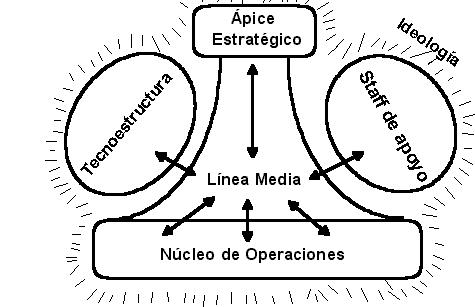
\includegraphics[width=0.5\textwidth]{aa1.jpg}
  \caption{Partes básicas de la organización}
  \label{aa1jpg}
\end{figure}

\begin{figure}[h!]
\centering
  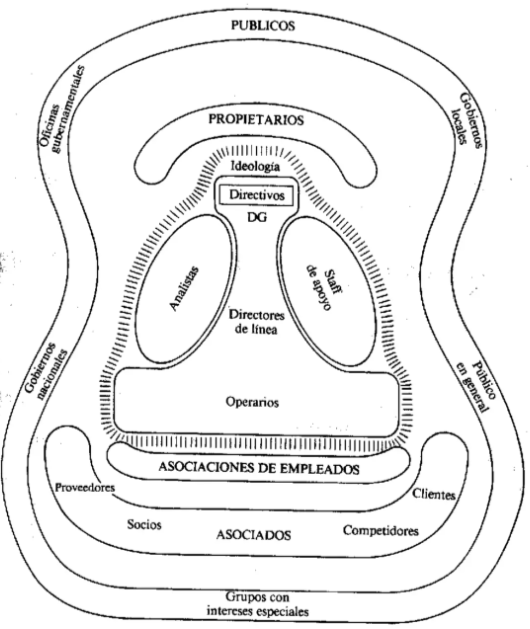
\includegraphics[width=0.5\textwidth]{aa2.png}
  \caption{Influencias internas y externas de una organización}
  \label{aa2}
\end{figure}
La forma característica es la forma empresarial, el cuadro administrativo delega en el, la construcción de la organización. Esta forma aparece al inicio de toda organización. 

Se quedan en esta configuración mientras que el directivo sigue en activo aunque haya disonancia cognitiva. Los fundadores son de personalidad fuerte y sus colaboradores guardan lealtad al fundador y quien los contrató.

Una empresas mueren otras evolucionan hacia otra configuración; que pasa con un ataque al corazón, algunos se fijan demasiado en detalle operativo; otros ponen demasiado énfasis en el contexto y si no hay mecanismo de autocorreción viene la defunción

Cuando falta el líder carismático y adorado, los seguidores tratan de institucionalizar ese carisma creando mitos como referentes a seguir.

Si se requiere de aplicación de conocimientos complejos pero estandarizados es algo \textbf{profesional}

Si es algo innovador no existe en algún otro lado.

las configuraciones maquinales suelen evolucionar como maquinal de sistema cerrado (madurez)

Lectura del mercado, retroalimentación directa, capacidad de aceptar errores, proceso de cambio, descongelar, cambiar o recongelar.

\subsubsection{Tramo de control}
El tramo de control se puede definir como el número de subordinados que un administrador puede dirigir con eficiencia y eficacia. Su importancia se refleja en que conforme un administrador ascendiente en una organización tiene que tratar con un mayor número de problemas no estructurados, de manera que los altos ejecutivos deben tener un tramo menor que los administradores de niveles medios.

En gran parte el tramo de control puede determinar el número de niveles y administradores que necesita una organización. Si todos los aspectos que se relacionan en el manejo de la empresa permanecen intactos, mientras más amplio sea el tramo de control, más eficiente es el diseño de la organización.

Para definir un eficiente y eficaz tramo de control, se deben tener en cuenta los siguientes aspectos:
\begin{itemize}
    \item La capacitación del administrador debe estar de acuerdo al tipo de objetivos que se pretendan obtener
    \item La experiencia es de vital importancia, ya que esta puede asegurar en un momento determinado la aplicación de correctivos inmediatos
    \item El establecimiento de tareas y responsabilidades deben ser perfectamente expuestos a cada uno de los subordinados
    \item La complejidad de las tareas debe ser evaluada para la contratación del personal idóneo
    \item El administrador debe ser uno de los que esté más familiarizado con los sistemas de información dentro de la empresa
    \item En el tramo de control debe definirse claramente los objetivos y los fundamentos de la cultura organizacional
    \item Por último debe fijarse el tipo de administración a la cual se quiere someter la empresa.
\end{itemize}
En la fijación del tupo de administración y tramo de control se pueden presentar dos tipos que tienen sus ventajas:

En un tramo estrecho, se presenta una supervisión estricta y alguna desventaja es en cuanto a los superiores que tienden a intervenir en el trabajo de los empleados, o se establecen demasiados niveles de administración (representando costos).

En los tramos amplios, los superiores se encuentran obligados a delegar funciones, planear o establecer políticas claras en el manejo administrativo o se seleccionan cuidadosamente a los subordinados; empero las desventajas son que se tienden a sobrecargar de trabajo a los administradores, se presenta pérdida temporal del control superior y se requiere una gran calidad en el manejo de la administración gerente.

Se han hecho diversos esfuerzos para determinar el tramo de administración ideal; uno de los primeros más importantes es del francés V.A. Graicunas (1937).

Los críticos sostuvieron que faltaron las relaciones organizacionales con terceras personas y también que este es el número posible de relaciones pero no es verdadero; asume que las relaciones ocurren con igual frecuencia y presuponen que las relaciones tienen igual intensidad
% \begin{equation}
%     R = n\left(\frac{2^n}{2}\right)
% \end{equation}
% Las relaciones potenciales entre un gerente y sus subordinados:
% \begin{align*}
%     \text{} M\Leftrightarrow  A\\
%     \text{}M\Leftrightarrow 
% \end{align*}

% La aportación de Graicunas puede tener limitaciones pero es de gran importancia como punto de partida

En 1967 Lawrence Paul R. y Lorsch Jay W. utilizaron el tramo de control promedio como una dimensión en la medición de la estructura organizacional. Ellos consideraron tramos de control de diez subordinados como un indicador de baja estructura y tramo de tres a cinco subordinados como el indicador de alta estructura.

Lindall F. Urwick fue autor de cuatro principios de administración y uno de  ellos el que se refiere al principio de la amplitud administrativa (span of control) menciona que ``cada superior no debe tener más que un cierto número de subordinados''. El superior no tiene sólo personas para supervisarlas sino también y principalmente las relaciones entre las personas que supervisa.

El caso de la corporación Lockheed constituye un ejemplo representativo del planteamiento formal para la determinación del os tramos óptimos de control; en esta organización se desarrolló un sistema de índice valorado que mide los principales factores de un tramo de control.

Hampton (1992), señala que en la serie de trabajos dedicados al estudio del tramo óptimo se han identificado como elementos que influyen en su diseño los siguientes:
\begin{itemize}
    \item Rutinización de las tareas
    \item Formalización de las tareas
    \item Número de ayudantes utilizados
    \item Ubicación geográfica de los subordinados
    \item Rotación de personal
    \item Estabilidad de las operaciones
    \item Necesidad de coordinación o de supervisión estrechas
    \item Tareas ajenas a la supervisión efectuadas por ellos
    \item Nivel de tecnología
    \item Capacitación de los subordinados
    \item Semejanzas de funciones cumplidas por los subordinados
    \item Autoevaluación de los gerentes sobre sus capacidades generales y globales como supervisores
\end{itemize}
La diferencia cultural en la delimitación del tramo de administración: ``Un estudio de empresas japonesas en USA reveló que los supervisores de primer nivel supervisaban un promedio de 15 empleados, las cifras de las compañías de USA era de 30. Se ha interpretado que la diferencia refleja la importancia relativamente mayor que los japoneses le dan al hecho de conocer a cada empleado, proceso que exige mayor esfuerzo y contacto''. El tramo de control es un principio importante de la organización, los que lo ignoran paga a menudo un precio muy alto (Urwik)

Mientras Koontz (1995) considera que la amplitud del tramo de administración depende de capacidades personales del administrador tales como comprender rápidamente, llevarse bien con los compañeros y ganarse su lealtad y respecto, la condición más importante es la habilidad del administrador para reducir el tiempo que pasas con los subordinados, por supuesto esto va a depender ed cada administrador, personal, y tareas pero de manera general las condicionantes del tramo de control son:

Poca o ninguna capacitación, delegación de autoridad inadecuada o confusa, planes confusos para operaciones no repetitivas, objetivo y estándares no verificables, cambios rápidos en los ambientes internos y externos, y subordinados inmaduros; uso de técnicas de comunicación deficientes o inadecuadas incluyendo instrucciones vagas, interacción ineficaz entre el supervisor y el subordinado reuniones ineficaces, mayor número de especialidades en los niveles inferiores y medio, administrador incompetente no capacitado, tarea compleja y renuncia de los subordinados asumiendo responsabilidades y riesgos razonables todo esto en los tramos estrechos.

Para los tramos amplios son la capacitación completa de los subordinados, delegación clara para realizar tareas bien definidas, planes bien definidos para operaciones repetitivas, objetivos verificables utilizados como estándares, cambios lentos en los ambientes internos y extremos; subordinados maduros; uso de técnicas apropiadas ales como la estructura de organización apropiada, comunicación escrita y oral, Interacción eficaz entre el superior y el subordinado reuniones eficaces, número de especialidades en los niveles superiores (los altos gerentes preocupados por el ambiente externo), administrador competente y capacitado, tareas sencilla, buena disposición de los subordinados asumiendo responsabilidades y riesgos razonables.

Con respecto al tramo óptimo no existe acuerdo, y lo que aquí se pretende es señalar que es de suma importancia el análisis del tipo de puesto, la capacitación de los subordinados, la capacidad de solución de problemas del supervisor, la claridad de los manuales de comportamiento, etc.

La motivación nos acerca a los objetivos; conocer las diferencias individuales del comportamiento humano y de qué manera influirán en el desempeño y eficacia.


































